\documentclass[12pt,fleqn]{article}\usepackage{../common}
\begin{document}
SVD ile Kumeleme

Tekil Deger Ayristirma (Singular Value Decomposition -SVD-) ile bir veri
madenciligi ornegi gorecegiz. Ornek olarak [1] adresinde tarif edilen /
paylasilan zaman serisini kullandik. Serinin tumunu kullanilmadi, ilk 10
noktasini aldik, ve grafige bakinca iki tane ana seri turu oldugunu
goruyoruz.

\begin{minted}{python}
data = np.genfromtxt("synthetic_control.data", dtype=float)

print data.shape

for t in data[:,0:10]: plot(t); hold(True)

plt.savefig('svd_2.png')
\end{minted}

\begin{verbatim}
(600, 60)
\end{verbatim}

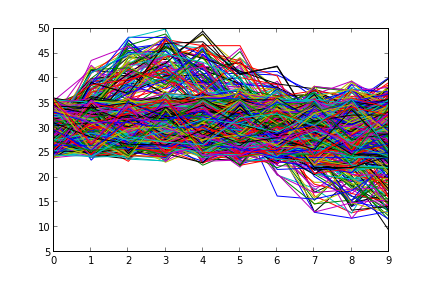
\includegraphics[height=6cm]{svd_2.png}

Peki bu serileri nasil otomatik olarak kumeleyerek bulurduk / birbirinden
ayirtederdik?  Lineer Cebir Ders 29'da SVD'nin matematigini
isledik. SVD bir matris $A$ uzerinde ayristirma yapar, ve $A$ herhangi
boyutta, turde bir matris olabilir.

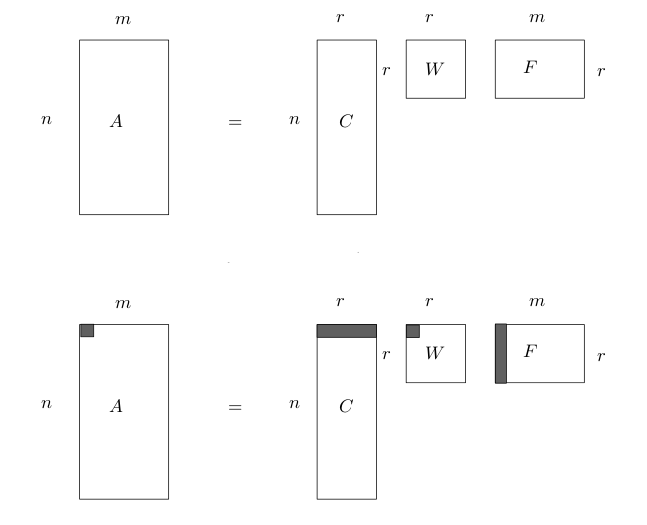
\includegraphics[height=7cm]{svd_1.png}


Ayristirma $m \times n$ boyutlu matrisi $A=CWF$ olarak ayristirir, burada
$C$, ana matris ile ayni miktarda satira sahiptir, $F$ ayni miktarda kolona
sahiptir. Ayristirma sonrasi $A$'nin kertesi (rank) $r$ ortaya cikar, eger
tum $A$ kolonlari birbirinden bagimsiz ise, o zaman $r=m$ olacaktir, ama
kolonlarin bazilari mesela ayni olcumu degisik katlarda tekrarliyor ise, o
zaman matriste tekillik vardir, ve bu durumda $r < m$ olur, ve ortadaki $W$
matrisi $r \times r$ oldugu icin beklenenden daha ufak boyutlarda
olabilir. 

Ayrica SVD, $W$ caprazindaki ozdegerleri buyukluk sirasina gore dizer, ve
her ozdegere tekabul eden ozvektorler de ona gore siraya dizilmis
olacaktir, ve SVD tamamlaninca mesela "en buyuk 10" ozdegere ait olan
$CWF$ degerlerini alip, digerlerini atmayi da secebiliriz, yani kerte
uzerinden yapilan "eleme" ustune bir eleme de kendimiz yapabiliriz. Bu
elemeyi yapabilmemizin mantigi soyle; kucuk ozdegerlerin carptigi
ozvektorlerin nihai toplama daha az etki ettigi soylenebilir, ve bu
"gurultuyu" elemek sonucu degistirmeyecektir. Ayrica bu elemeyi yaparak
bir tur boyut azaltma (dimensionality reduction) islemini de ayni zamanda
basarmis oluruz.

Ayristirmanin Anlamlari

Bir ayristirmayi degisik sekillerde gormek mumkundur. Bunlardan onemli
birisi cizge bakis acisidir (graph interpretation). Cizge bilindigi gibi
dugumler ve onlar arasindaki ayritlardan (edges) olusur. Bir cizge matris
formunda temsil edilebilir, satir / kolon kesisimi iki dugum arasindaki
ayritin agirligini, ya da varligini (1 ve 0 uzerinden) temsil edecektir. Bu
durumda SVD sonucunda elde edilen $CWF$, bize iki dugum arasi gecisli
(bipartite) cizgeyi, uc dugum arasi gecisli (tripartite) cizgeye cevrilmis
halde geri verir. Ve bu yeni cizgede en fazla $r$ tane gecis noktalari
(waystations) olusmustur, ustte bahsettigimiz eleme ile gecisler daha da
azaltilabilir. 

Simdi, bu gecis noktalarina olan $C$'nin ``baglanma sekli'', "baglanma
kuvveti", ek kumeleme basamagi tarafindan kullanilabilir. Bu
"azaltilmis" gecisin uzerindeki her islem / ona yapilan her referans
kumeleme icin bir ipucudur. Bunu gormek icin ornek zaman serilerinin
SVD sonrasi elde edilen $C$ (ornekte \verb!u!) matrisinin ilk
iki kolonunu bile grafiklemek yeterlidir.

\begin{minted}{python}
import scipy.linalg as lin
data = np.genfromtxt("synthetic_control.data", dtype=float)

# before norm, and take only 10 data points
data = data[:,0:10]

print data.shape

# show the mean, and std of the first time series
print data[0,:]
print np.mean(data[0,:], axis=0)
print np.std(data[0,:], axis=0)

# normalize
data -= np.mean(data, axis=0)
data /= np.std(data, axis=0)

# after norm
print data[0,:]

u,s,v = lin.svd(data, full_matrices=False)
print 'svd'
print u.shape
print s
print v.shape

plt.plot(u[:,0], u[:,1], '.')
plt.savefig('svd_3.png')
\end{minted}

\begin{verbatim}
(600, 10)
[ 28.7812  34.4632  31.3381  31.2834  28.9207  33.7596  25.3969  27.7849
  35.2479  27.1159]
30.40918
3.16894521278
[-0.35501371  0.85457443 -0.10641642 -0.16202975 -0.51986031  0.56762802
 -1.19371757 -0.29304061  1.27639519 -0.2095089 ]
svd
(600, 10)
[ 48.29293361  30.97232928  24.52860861  20.63081553  20.0940039
  17.52035809  16.48932523  16.03796372  15.41270426  14.27678793]
(10, 10)
\end{verbatim}

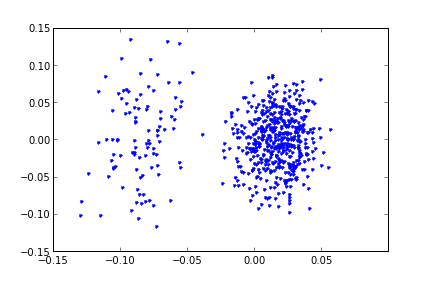
\includegraphics[height=6cm]{svd_3.png}

Goruldugu gibi net bir sekilde iki tane kume ortaya cikti. Bu kumeler
yazinin basindaki iki ayri zaman serisi obeklerine tekabul ediyorlar. 

O zaman serilerini ayirtetmek icin ne yapariz? Ustteki veriler uzerinde
kmeans isletebilirdik, ya da kabaca bakiyoruz, dikey olarak -0.025
seviyesinde bir cizgi ayirac olarak gorulebilir. Numpy filtreleme teknigi

\verb!u[:,0] < -0.025!

bize ana veri uzerinde uygulanabilecek \verb!True! ve \verb!False!
degerleri verir, bunlari alarak ana veriye filtrele olarak uygulariz,

\verb!data[u[:,0] < -0.025]!

ve mesela birinci kumeye ait zaman serilerini bulabiliriz. 

Kontrol etmek icin ilk 3 kolonun degerlerini uc boyutta grafikleyelim.

\begin{minted}{python}
from mpl_toolkits.mplot3d import Axes3D
import scipy.linalg as lin

data = np.genfromtxt("synthetic_control.data", dtype=float)

data = data[:,0:10]

print data.shape

data -= np.mean(data, axis=0)
data /= np.std(data, axis=0)

u,s,v = lin.svd(data)
print 'svd'
print u.shape
print s
print v.shape

fig = plt.figure()
ax = Axes3D(fig)
ax.plot(u[:,0], u[:,1], u[:,2],',', zs=0, zdir='z', label='zs=0, zdir=z')
plt.savefig('svd_4.png')
\end{minted}

\begin{verbatim}
(600, 10)
svd
(600, 600)
[ 48.29293361  30.97232928  24.52860861  20.63081553  20.0940039
  17.52035809  16.48932523  16.03796372  15.41270426  14.27678793]
(10, 10)
\end{verbatim}

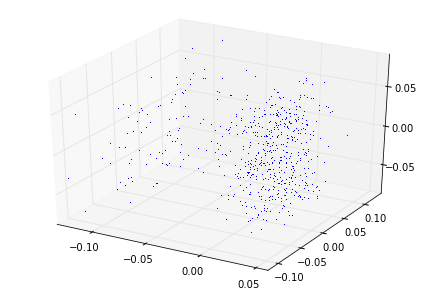
\includegraphics[height=6cm]{svd_4.png}

Yine iki tane kume oldugunu goruyoruz. 

Simdi biraz daha degisik bir probleme bakalim, bu sefer bir grup kelimeyi
birbirlerine benzerlikleri (ya da uzakligi) uzerinden kumelemeye ugrasacagiz. 

Benzerlik, Levenhstein mesafesi adli olcut [2] uzerinden olacak. Matrisimiz
her kelimenin her diger kelime ile arasindaki uzakligi veren bir matris
olmali, eger 100 kelime var ise, bu matris 100 x 100 boyutlarinda
olacak. SVD sonrasi elde edilen \verb!u! uzerinde kmeans isletecegiz, ve
kumeleri bulacagiz. Ayrica her kume icin bir ``temsilci'' secebilmek icin
kmeans'in bize verdigi kume ortasi kordinatinin en yakin oldugu kelimeyi
cekip cikartacagiz, ve onu temsilci olarak alacagiz.

Kelime mesafesi olarak

\begin{minted}{python}
def levenshtein(s1, s2):
  l1 = len(s1)
  l2 = len(s2)

  matrix = [range(l1 + 1)] * (l2 + 1)
  for zz in range(l2 + 1):
    matrix[zz] = range(zz,zz + l1 + 1)
  for zz in range(0,l2):
    for sz in range(0,l1):
      if s1[sz] == s2[zz]:
        matrix[zz+1][sz+1] = min(matrix[zz+1][sz] + 1, matrix[zz][sz+1] + 1, matrix[zz][sz])
      else:
        matrix[zz+1][sz+1] = min(matrix[zz+1][sz] + 1, matrix[zz][sz+1] + 1, matrix[zz][sz] + 1)
  return matrix[l2][l1]

s1 = "pizza"
s2 = "pioazza"   
distance = levenshtein(s1, s2)       
print 'The Levenshtein-Distance of ',s1, ' and ', s2, ' is ', distance

s1 = "hamburger"
s2 = "haemmurger"   
distance = levenshtein(s1, s2)       
print 'The Levenshtein-Distance of ',s1, ' and ', s2, ' is ', distance
\end{minted}

\begin{verbatim}
The Levenshtein-Distance of  pizza  and  pioazza  is  2
The Levenshtein-Distance of  hamburger  and  haemmurger  is  2
\end{verbatim}

\begin{minted}{python}
import scipy.linalg as lin
from sklearn.cluster import KMeans
import itertools

words = np.array(
    ['the', 'be', 'to', 'of', 'and', 'a', 'in', 'that', 'have',
     'I', 'it', 'for', 'not', 'on', 'with', 'he', 'as', 'you',
     'do', 'at', 'this', 'but', 'his', 'by', 'from', 'they', 'we',
     'say', 'her', 'she', 'or', 'an', 'will', 'my', 'one', 'all',
     'would', 'there', 'their', 'what', 'so', 'up', 'out', 'if',
     'about', 'who', 'get', 'which', 'go', 'me', 'when', 'make',
     'can', 'like', 'time', 'no', 'just', 'him', 'know', 'take',
     'people', 'into', 'year', 'your', 'good', 'some', 'could',
     'them', 'see', 'other', 'than', 'then', 'now', 'look',
     'only', 'come', 'its', 'over', 'think', 'also', 'back',
     'after', 'use', 'two', 'how', 'our', 'work', 'first', 'well',
     'way', 'even', 'new', 'want', 'because', 'any', 'these',
     'give', 'day', 'most', 'us'])

print "calculating distances..."

(dim,) = words.shape

f = lambda (x,y): levenshtein(x,y)

res=np.fromiter(itertools.imap(f, itertools.product(words, words)),
                dtype=np.uint8)
A = np.reshape(res,(dim,dim))

print "svd..."

u,s,v = lin.svd(A, full_matrices=False)

print u.shape
print s.shape
print s
print v.shape

data = u[:,0:8]
k=KMeans(init='k-means++', n_clusters=25, n_init=10)
k.fit(data)
centroids = k.cluster_centers_
labels = k.labels_
print labels

def dist(x,y):   
    return np.sqrt(np.sum((x-y)**2, axis=1))
    
print "clusters, centroid points.."
for i,c in enumerate(centroids):
    idx = np.argmin(dist(c,data[labels==i]))
    print words[labels==i][idx]
    print words[labels==i]
    
plt.plot(centroids[:,0],centroids[:,1],'x')
plt.hold(True)
plt.plot(u[:,0], u[:,1], '.')
plt.savefig('svd_5.png')

from mpl_toolkits.mplot3d import Axes3D
fig = plt.figure()
ax = Axes3D(fig)
ax.plot(u[:,0], u[:,1], u[:,2],'.', zs=0,
        zdir='z', label='zs=0, zdir=z')
plt.savefig('svd_6.png')
\end{minted}

\begin{verbatim}
calculating distances...
svd...
(100, 100)
(100,)
[  3.57988202e+02   4.64912561e+01   3.21352688e+01   2.38031643e+01
   2.14888993e+01   1.75355875e+01   1.72577475e+01   1.50823345e+01
   1.36053187e+01   1.27864289e+01   1.20850058e+01   1.09366461e+01
   1.02722223e+01   9.15906107e+00   8.93781797e+00   8.08808906e+00
   7.55885762e+00   7.38765898e+00   7.03189413e+00   6.37905207e+00
   6.08100883e+00   5.93978699e+00   5.80476820e+00   5.48573127e+00
   4.93815941e+00   4.58515335e+00   4.40072056e+00   4.10393093e+00
   3.82184278e+00   3.62002998e+00   3.52076475e+00   3.21765568e+00
   3.19448751e+00   2.97591545e+00   2.90604264e+00   2.82566873e+00
   2.75236845e+00   2.51068720e+00   2.46909289e+00   2.39525952e+00
   2.31057708e+00   2.17681774e+00   2.11768873e+00   2.02116412e+00
   1.99158340e+00   1.84283752e+00   1.80985462e+00   1.73585790e+00
   1.59395705e+00   1.57675090e+00   1.49638568e+00   1.49354064e+00
   1.40623601e+00   1.40412600e+00   1.24442892e+00   1.23842955e+00
   1.22119742e+00   1.20466658e+00   1.19604521e+00   1.08815700e+00
   9.78864620e-01   9.71322173e-01   8.83519026e-01   8.53898791e-01
   8.53690716e-01   7.32954748e-01   7.14196035e-01   6.92366775e-01
   6.83931613e-01   5.88533124e-01   5.45586737e-01   5.01747612e-01
   4.90740691e-01   4.29689160e-01   4.09996636e-01   4.03042824e-01
   3.80587104e-01   3.48811148e-01   3.28580353e-01   3.25050141e-01
   3.09318382e-01   2.39526940e-01   2.29926274e-01   1.96030630e-01
   1.86987383e-01   1.46740385e-01   1.44728633e-01   1.30118418e-01
   1.28613583e-01   8.03675410e-02   6.31950264e-02   5.25562558e-02
   3.08220025e-02   2.85652995e-02   2.84199001e-02   4.43547511e-03
   1.60953158e-04   3.44433012e-14   3.44433012e-14   3.44433012e-14]
(100, 100)
[ 4 13  1 19  8 22 10 21 12  2 10 19 19 19  0 13 22 19  1 22 18 17 10  2 15
  4 13  8 23 13 19  8  0  2  7  8 14 23 23 21  1  2 17 10  5 11  2  0  1 13
  7 12  8  6  6  1  5 11 15 12 24 11  3 19 15  9 14  4 13 23 21  4  1 15 20
  9 10  7 18  5  8  3 13  1  1 17 15  5 20  8  7  7  8 16  8 18  6  8  5  2]
clusters, centroid points..
with
['with' 'will' 'which']
do
['to' 'do' 'so' 'go' 'no' 'now' 'two' 'how']
I
['I' 'by' 'my' 'up' 'get' 'us']
year
['year' 'after']
them
['the' 'they' 'them' 'then']
most
['about' 'just' 'also' 'first' 'most']
like
['like' 'time' 'give']
even
['one' 'when' 'over' 'even' 'new']
any
['and' 'say' 'an' 'all' 'can' 'back' 'way' 'want' 'any' 'day']
come
['some' 'come']
if
['in' 'it' 'his' 'if' 'its']
into
['who' 'him' 'into']
have
['have' 'make' 'take']
be
['be' 'he' 'we' 'she' 'me' 'see' 'use']
would
['would' 'could']
good
['from' 'know' 'good' 'look' 'work']
because
['because']
out
['but' 'out' 'our']
this
['this' 'think' 'these']
for
['of' 'for' 'not' 'on' 'you' 'or' 'your']
only
['only' 'well']
that
['that' 'what' 'than']
at
['a' 'as' 'at']
other
['her' 'there' 'their' 'other']
people
['people']
\end{verbatim}

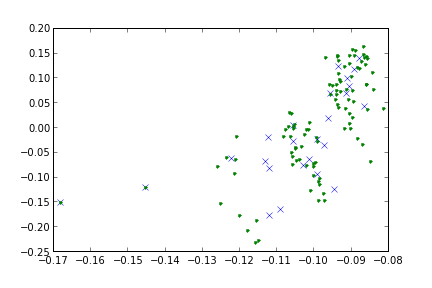
\includegraphics[height=6cm]{svd_5.png}

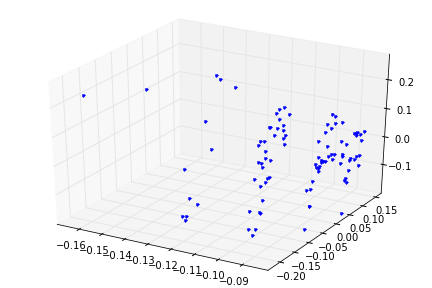
\includegraphics[height=6cm]{svd_6.png}


Bu teknigin uygulanabilecegi daha pek cok alan var. Mesela her dokumanin
icindeki belli kelimelerin sayilari kolonlarda (her kolon ozel bir kelimeye
tekabul edecek sekilde), ve dokumanlarin kendisi satirlarda olacak sekilde
bir matrisimiz olsaydi, SVD bu matris uzerinde de bir kumeleme icin
kullanilabilirdi. Bu ornekte ``kac tane kelime oldugu'' gibi bir olcut
vardir (daha once kelimelerin birbirine uzakligini kullandik), ama teknik
yine de ise yarar.

Not: \verb!np.fromiter .. itertools.imap! kullanimini anlamak
icin [4]'e bakilabilir.

[1] \url{kdd.ics.uci.edu/databases/synthetic_control/synthetic_control.data.html}

[2] \url{sayilarvekuramlar.blogspot.de/2012/07/kelime-benzerligi-levenshtein-mesafesi.html}

[3] Skillicorn, D., Understanding Complex Datasets Data Mining with Matrix Decompositions

[4] \url{sayilarvekuramlar.blogspot.de/2012/07/dongu-yazmamak-fonksiyonel-diller-python.html}



\end{document}
